\part*{Introduction}
\label{introduction}
\markright{}
\addcontentsline{toc}{part}{Introduction}
\par
Ce projet s'inscrit dans le cadre d'une demande de \textsc{Mme. Guiziou}, doctorante en biologie, recherchant l'aide de l'informatique afin d'approfondir ses recherches en matière d'approche logique de l'ADN.

\par
L'ADN est composé de bases, briques élémentaires du vivant, dont certains groupements correspondent à une fonction particulière : promouvoir un gène, l'activer, etc. Et plusieurs fonctions à la suite forment ainsi des mots, grandes portions de l'ADN, ayant une sémantique précise.

\begin{wrapfigure}{r}{0.4\textwidth}
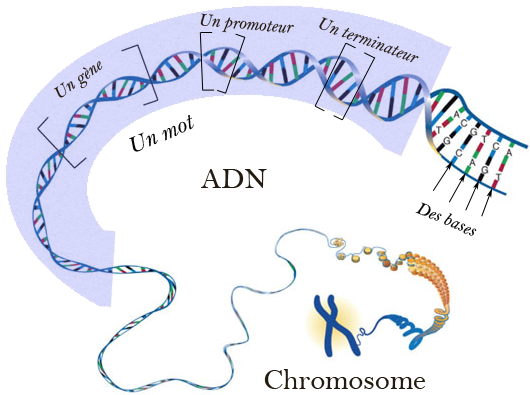
\includegraphics[width=0.4\textwidth]{1b}
\end{wrapfigure}

\par
L'information véhiculée par la sémantique de ces mots, selon leur environnement, entraîne l'exécution de telle ou telle tâche. Cette analogie entre code génétique et logique est le sujet de nombreuses recherches, néanmoins il n'existe pas encore de formalisme complet dans ce domaine.

\par
L'étude de cette logique de l'ADN nécessite la synthèse de matériel génétique. Cependant, celle-ci est coûteuse en temps et en argent. Tout le problème réside donc dans la recherche de mots simples et optimaux.

\par
Dans le cadre du projet, il fut dans un premier temps nécessaire de trouver quelle fonction logique implémentait un mot donné.

\par
Dès lors, la suite fut de s'intéresser à la réciproque : quels étaient les mots implémentant une fonction logique donnée ? Notre approche fut celle de la génération de masse passant par la création d'un très grand nombre de mots que l'on savait représentatif de l'ensemble des mots possibles.

\par
La création puis le parcours d'une base de donnée de mots a été notre dernière contribution au projet et nous a permis de répondre à la question dans une certaine mesure.